\documentclass[usenatbib]{mnras}
\usepackage{graphicx}
\usepackage{bm}
\usepackage{amsmath}
\usepackage{amssymb}
\usepackage{algorithm}
\usepackage{algpseudocode}
\usepackage{caption}
\usepackage{subcaption}
\usepackage{layouts}
\usepackage{cleveref}
\usepackage{txfonts}
\usepackage[T1]{fontenc}

\newcommand{\logL}{\{ \log \Like_i \}}
\newcommand{\thetab}{\bm{\theta}}
\newcommand{\logLm}{\log \Like_\mathrm{max}}
\newcommand{\set}[1]{\{#1\}}
\newcommand{\nlive}{n_\mathrm{live}}
\newcommand{\Like}{\mathcal{L}}
\newcommand{\DKL}{\mathcal{D}_\mathrm{KL}}



\title[Approximating the end of nested sampling]{Approximating the end of nested sampling}
\author[Z. Hu et. al]{Zixiao Hu, Artyom Baryshnikov, Will Handley}


\begin{document}
\label{firstpage}
\pagerange{\pageref{firstpage}--\pageref{lastpage}}
\maketitle


\begin{abstract}
This paper develops a technique to estimate the runtime of a nested sampling run at an intermediate iteration for any nested sampler. The known likelihood at an iteration is fitted, then extrapolated using a Gaussian model likelihood, which allows the remaining evidence and prior volume at termination to be calculated. We find that the method succesfully recovers the true endpoint within standard error from the beginning for near-Gaussian likelihoods. For non-Gaussian likelihoods, the estimate is still the correct order of magnitude and converges to the correct answer by the end of the run. 
\end{abstract}

\begin{keywords}
methods: data analysis -- methods: statistical
\end{keywords}

\section{Introduction}
Users would like a order of magnitude runtime estimate
Figure of PolyChord output



\section{Background}
\subsection{Notation}
We shall begin with a brief description of nested sampling to establish the necessary notation. For a given likelihood $\Like(\theta)$ and prior $\pi(\theta)$, nested sampling simultaneously calculates the Bayesian evidence
\begin{equation}\label{eq:evidence}
	\mathcal{Z} = \int \Like(\theta)\ \pi(\theta)\ \mathrm{d}\theta
\end{equation}
while producing samples of the posterior distribution 
\begin{equation}
	\mathcal{P}(\theta) = \frac{\Like(\theta) \pi(\theta)}{\mathcal{Z}}.
\end{equation}
The algorithm operates by maintaining a set of $\nlive$ \textit{live points} sampled from the prior, which can vary in number throughout the run. At each iteration, the point with the lowest likelihood is removed and added to a list of \textit{dead points}. A new point is then drawn from the prior, subject to the constraint that it must have a higher likelihood than the latest dead point. Repeating the procedure leads to the live points shrinking around peaks in the likelihood. 
\par
The integral in \cref{eq:evidence} is then evaluated by transformation to a one-dimensional integral over the \textit{prior volume} $X$, defined as
\begin{equation}
	\mathcal{Z} = \int_0^1 \Like(X)\ \mathrm{d}X \approx \frac{1}{2}\sum_{i=1} \Like_i (X_{i-1}-X_{i+1}),
\end{equation}
where $X(\Like)$ is the fraction of the prior greater than $\Like$. The prior volumes $X_i$ are unknown, but can be statistically estimated as follows: one can define a \textit{shrinkage factor} $t_i$ at each iteration $X_{i} = t_i X_{i-1}$, such that
\begin{equation}
	X_i = \prod_{k=1}^i t_k.
\end{equation}
The $t_i$ are the maximum of $\nlive$ points drawn from $[0,1]$, so follow the distribution
\begin{equation}\label{eq:t_dist}
	p(t_i) = \nlive t_i^{\nlive-1}, \quad \mathrm{E}[\log t_i] = -\frac{1}{\nlive}, \quad \mathrm{Var}[\log t_i] = \frac{1}{\nlive^2}.
\end{equation}
The algorithm terminates when an user-specified condition is met; a popular choice is to terminate when the evidence in the live points falls below some fraction $\epsilon$ of the accumulated evidence e.g. $10^{-3}$. The remaining live points are then killed off one by one without replacement and added to the evidence. 
\par
Uncertainties in the evidence are dominated by the spread in the prior volume distribution, and the simplest way to estimate them is by Monte Carlo sampling over sets of $\bm{t}$. 


\section{Convergence of a nested sampling run}
Let us now take a top-down view of a nested sampling run as it progresses to observe how it converges. 

\subsection{Posterior convergence}
We will examine how our set of samples evolve over the course of a nested sampling run. The conventional perspective for the progress of a run is with $\log X$ along the x-axis; the prior volume is compressed at a steady rate, only picking up the bulk of the integral/posterior at around $\log X = \DKL$.  
\par
At an intermediate iteration, we have an accurate reconstruction of the posterior only down to the current prior volume $\log X_*$. The live points contain information below this volume, but not much more. If we kill off all the live points as if we were terminating, then by \cref{eq:t_dist} the prior volume of the final live point $\log X_\mathrm{min}^{\mathrm{live}}$ has mean and variance
\begin{equation}
	\mathrm{E}[\log X_\mathrm{min}^{\mathrm{live}}] = \mathrm{E}[\log X_*] - \sum_{k=1}^{\nlive} \frac{1}{n_k} \approx -\frac{i_*}{\nlive} - \log \nlive - \gamma,
\end{equation}
\begin{equation}
	\mathrm{Var}[\log X_\mathrm{min}^{\mathrm{live}}] = \mathrm{Var}[\log X_*] + \sum_{k=1}^{\nlive} \frac{1}{n_k^2} \approx \frac{i}{\nlive^2} + \frac{\pi^2}{6},
\end{equation}
where the large $\nlive$ limit is taken for the approximation and $\gamma$ is the Euler-Mascheroni constant. 
\par
This shows that the live points only get us a factor of $\log \nlive$ closer to the posterior bulk, or in other words, it is not until we are around $\log \nlive$ away from $\log X = \DKL$ that the samples begin to resemble the posterior. Intuitively, if the likelihood is sharply peaked then for most of the run the live points are too diffuse to land there with any significant probability.
\par
\begin{figure}
\begin{center}
	\includegraphics{figures/live_point_distribution.pdf}
\end{center}
\caption{}
\label{fig:}
\end{figure}


\subsection{Loglikelihood convergence}
We now offer an alternate view of the convergence of a nested sampling run, via the loglikelihood instead of the prior volumes. To get an insight into the analytics, work with a Gaussian likelihood of $d$ dimensions and a lengthscale of $\sigma$;
\begin{equation}\label{eq:logL}
	\log\Like = \log\Like_\mathrm{max} - \frac{X^{2/d}}{2\sigma^2}.
\end{equation}
The distribution of the true posterior in $\log\Like$ is
\begin{equation}
    P(\log\mathcal{L}) = \frac{1}{\Gamma(\frac{d}{2})}e^{\log\mathcal{L}-\log\mathcal{L}_\mathrm{max}} (\log\mathcal{L}_\mathrm{max}-\log\mathcal{L})^{\frac{d}{2}-1}
\end{equation}
i.e. $2(\log\mathcal{L}_\mathrm{max}-\log\mathcal{L}) \sim \chi^2_{d}$, which is the same distribution as that of the dead points up to the latest dead likelihood $\log \Like_*$. Meanwhile, the live points are uniformly distributed over the constrained prior and hence have probability distribution
\begin{equation}
	P(\log\mathcal{L}) = \frac{d}{2}\frac{(\log\mathcal{L}_\mathrm{max}-\log\mathcal{L})^{\frac{d}{2}-1}}{(\log\mathcal{L}_\mathrm{max}-\log\mathcal{L}_*)^{\frac{d}{2}}} \quad [\log\Like_* < \log\Like <\log\Like_\mathrm{max}],
    \label{eq:PL}
\end{equation}
It is helpful at this stage to define a parameter
\begin{equation}
    y = \frac{\log\mathcal{L}-\log\mathcal{L}_*}{\log\mathcal{L}_\mathrm{max}-\log\mathcal{L}_*} 
    \label{eq:y}
\end{equation}
as a normalised measure of how far a point is between the latest dead point and the maximum loglikelihood, with $y=0$ corresponding to $\mathcal{L}_*$ and $y=1$ to $\mathcal{L}_\mathrm{max}$, so that
\begin{equation}
    P(y) = \frac{d}{2}(1-y)^{\frac{d}{2}-1} \quad [0<y<1].
    \label{eq:Py}
\end{equation}
We now seek the distribution for the maximum likelihood of the live points, $\log\Like_\mathrm{max}^{\mathrm{live}}$. Using the result that the maximum of $n$ variables with cumulative distribution $F(y)$ follows $\frac{d}{dy}( 1- (1-F(y))^n)$, we obtain
\begin{equation}
    P(y_\mathrm{max}^\mathrm{live}) = \frac{nd}{2}(1-y_\mathrm{max}^\mathrm{live})^{\frac{d}{2}-1}\left(1-(1-y_\mathrm{max}^\mathrm{live})^{\frac{d}{2}}\right)^{n-1}[0<y_\mathrm{max}^\mathrm{live}<1],
    \label{eq:Pyhat}
\end{equation}
which in the limit of large live points and dimensions can be roughly summarised by
\begin{equation}\label{eq:ylivemax}
	    \lim_{d,n\to\infty} y_\mathrm{max}^\mathrm{live} \sim \frac{2\log n}{d} \pm \sqrt{\frac{2}{3}}\frac{\pi}{d}.
\end{equation}
This shows that in general the live points are nowhere near the maximum loglikelihood at any iteration, though they do steadily squeeze the interval $[\log\mathcal{L}_*,\log\mathcal{L}_\mathrm{max}]$. In particular, in high dimensions $n$ only gets us harmonically/logarithmically closer, whilst $d$ pushes us linearly further away.
\par
This remains true even at the end of the nested sampling run. To see this, we write the halting condition as:
\begin{equation}
    f = \frac{\int_0^{X_\mathrm{end}} \mathcal{L} dX}{\int_0^\infty \mathcal{L} dX}.
    \label{eq:fint}
\end{equation}
Note that we have assumed that prior effects are negligible (so $1=\infty$), and that $f \ll 1$ so that the denominator is approximately the accumulated evidence. Computing this for \cref{eq:logL} we find the answer in terms of lower incomplete gamma functions
\begin{equation}
    f = 1- \frac{\Gamma_{d/2}\left(\frac{X_\mathrm{end}^{2/d}}{2\sigma^2}\right)}{\Gamma\left(\frac{d}{2}\right)}.
    \label{eq:f}
\end{equation}
Taking the $X_\mathrm{end}\ll (\sqrt{2}\sigma)^d$ limit (almost certainly valid at termination) we find
\begin{equation}
    \lim_{X_\mathrm{end}\ll (\sqrt{2}\sigma)^d} f \approx \frac{X_\mathrm{end}}{(\sqrt{2}\sigma)^d\Gamma(1+\frac{d}{2})} = \frac{(\log\mathcal{L}_\mathrm{max}-\log\mathcal{L}_\mathrm{end})^{\frac{d}{2}}}{\Gamma(1+\frac{d}{2})}.
\end{equation}
We thus have an expression relating $\mathcal{L}_\mathrm{end}$ at termination to the termination fraction $f$. This becomes yet more pleasing in the large $d$ limit, since $f^{2/d}\to 1$, we find via a Stirling approximation:
\begin{equation}
    \lim_{d\to\infty} \log\mathcal{L}_\mathrm{end} \approx \log\mathcal{L}_\mathrm{max} - \frac{d}{2e}.
\end{equation}
In the event that we keep $f$ in, we replace $\frac{d}{2e}\to \frac{d}{2e}f^{2/d}$, so we can of course battle the $\frac{d}{2e}$ term, but this becomes exponentially difficult in high dimensions.

\subsection*{Observation 3: nested sampling as a maximiser}
Putting this together, taking $\mathcal{L}_*$ in \cref{eq:y} to be $\mathcal{L}_\mathrm{end}$, and combining this with \cref{eq:ylivemax} we find
\begin{equation}
    \boxed{
        \log{\mathcal{L}}_\mathrm{max}^\mathrm{live} \approx \log\mathcal{L}_\mathrm{max} - \frac{d}{2e} + \frac{\log n}{e} \pm \frac{\pi}{\sqrt{6}e}
    },
\end{equation}
showing that in general nested sampling will finish at a contour $d/2e$ away from the maximum loglikelihood, and the final set of $n$ live points can get you $\log (n)/2e$ closer, with a chance of getting $\sim\pi/\sqrt{6}e=0.472$ closer still by statistical fluctuation.
\begin{figure*}
\begin{center}
	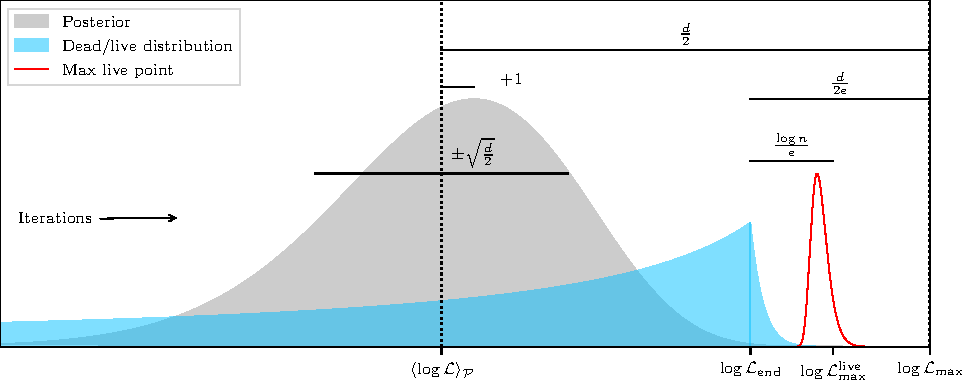
\includegraphics{figures/anatomy.pdf}
\end{center}
\caption{}
\label{fig:anatomy}
\end{figure*}
\par
From above analysis we learn that
\begin{itemize}
	\item Knowledge of the posterior early on in the run is limited by the maximum live point, which is far from the posterior bulk
	\item At termination, the maximum live point is far from the true maximum --> nested sampling alone is a poor optimiser (but great for finding starting point of gradient descent)
\end{itemize}



\section{Method}
Let us now tackle the problem of estimating how many steps we still have to take in a nested sampling run before we can terminate.
\par
The above analysis shows that our knowledge of the posterior at an intermediate iteration is limited by the maximum live point, which until just before the end is quite far from the posterior bulk. However, we can get an approximate image of the full posterior ahead of time, simply by \textit{extrapolating} the known likelihood profile; that is, the trajectory of $\Like(X)$ traced out by the live and dead points. 
\par
For practical purposes, one would never use this approximate posterior to do inference. However, it is more than sufficient for making a prediction for roughly how much evidence remains, and hence the point at which the run should terminate. Quantitatively, this proceeds as follows: fitting a model function $f(X, \thetab)$ to the known likelihood profile allows us to express the prior volume we need to compress to as 
\begin{equation}
	\Delta \mathcal{Z} = \epsilon \mathcal{Z}_\mathrm{tot},
\end{equation}
\begin{equation}\label{model endpoint}
	\int_0^{X_f} f(X, \thetab)\ dX = \epsilon \left( \int_0^{X_i} f(X, \thetab)\ dX + Z_\mathrm{dead} \right),
\end{equation}
where $X_i$ is the volume of the iteration we have currently compressed to, and $\mathcal{Z}_\mathrm{dead}$ is the evidence we have accumulated up to this point. $X_f$ can then be identified by solving the above equation either analytically or numerically. If $\nlive$ is constant then at each iteration $\log X$ decreases by $1/\nlive$, so the total number of iterations $N_f$ will be
\begin{equation}
	N_f = - \nlive \log X_f .
\end{equation}
One has freedom to choose the form of the fitting function $f(X, \thetab)$. Following the previous analysis, we use a Gaussian profile, which has the advantage that the regression itself can be sped up analytically, as well as the fact that many real likelihoods are Gaussian or near-Gaussian. However, any other function that is sufficiently flexible to capture the shape of the likelihood profile will do.

Fit a Gaussian profile, with advantages that a) Gaussian error common b) analytic optimisation 
Extraction of termination logX
Prediction uncertainty dominated by correlations, not least squares i.e. scatter of individual points - get by simulating X


\section{Results}
Toy examples - pure Gaussian,  wedding cake, Cauchy
Real cosmological examples - Planck


\end{document}

